\chapter{A estratégia de produção}
\label{chap:estrategia_da_producao}
%Neste capítulo será explicado como formular a estratégia de produção de uma empresa industrial visando atender o seu objetivo geral de desempenho. Uma estratégia de produção consiste em converter as intenções contidas em ações práticas como projetos concretos, planos e melhorias. Para isso, será explicado como a matriz "importância x desempenho" pode auxiliar na definição de estratégias de produção.

A estratégia de produção analisa o processo global da função de produção da empresa industrial como um todo. Por isso, caso exista, ela se preocupa com as outras partes da corporação, com as unidades de negócio (marketing, finanças, recursos humanos, entre outras) e com o local onde o negócio esta inserido (concorrentes, clientes externos, etc). Além disso, tem o objetivo de manter a área de operações adaptadas às mudanças externas como fatores ambientais dentre outros. Logo, a operação terá maiores chances de enfrentar os problemas futuros. Com isso, é mais garantido que as organizações possam ter níveis sustentáveis de vantagens competitivas \cite{correa2000administracao}.

Ainda segundo o autor, a matriz \textit{importância $\times$ desempenho}, mostrada na Figura \ref{fig:matriz_importancia_desempenho}, é uma ferramenta que deve ser utilizada para a priorização dos objetivos da função de operações. Essa matriz, possui duas dimensões: uma delas refere-se à importância relativa dada pelos clientes aos critérios de desempenho, utilizando a escala de nove pontos e a outra envolve uma classificação, também com uma escala de nove pontos, do desempenho de cada objetivo contra os níveis de desempenho atingidos pelos concorrentes.

\begin{figure}[H]
  \caption{Matriz importância $\times$ desempenho}
  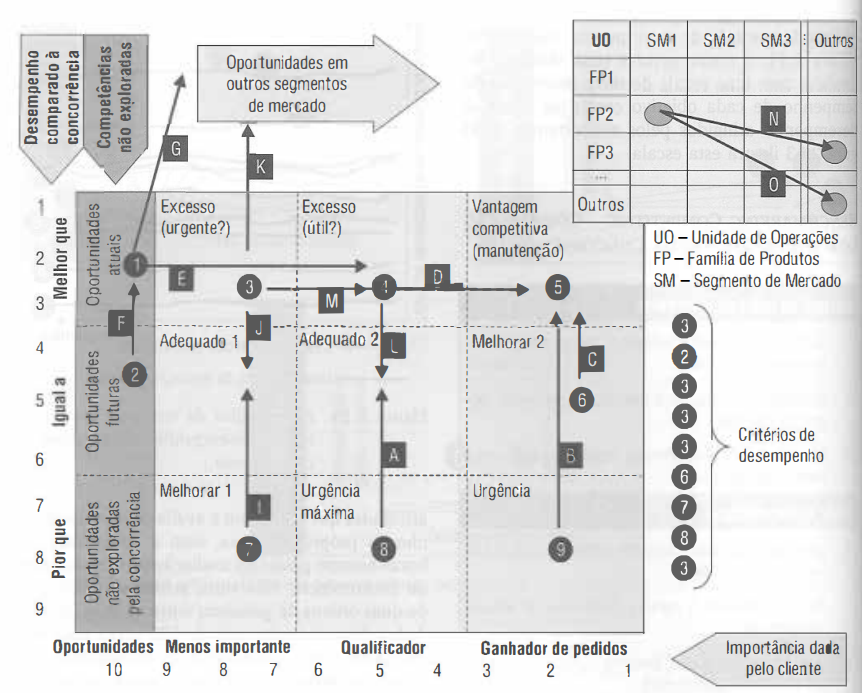
\includegraphics[width =1\textwidth]{images/impor_desem.png}
  \label{fig:matriz_importancia_desempenho}
  \caption*{Fonte: \cite{correa2000administracao}}
\end{figure}

O cruzamento das duas dimensões (importância dos critérios para o mercado e desempenho nos critérios comparado à concorrência) permite identificar regiões específicas na matriz, conforme mostrado na Figura \ref{fig:matriz_importancia_desempenho}. Esta traz uma arranjo eficaz no que se refere a estabelecerem prioridades e a partir disso, designar os esforços e recursos de melhoria estratégica em operações. Vale salientar que para se obter esta matriz é necessário ter em vista a análise de um dado conjunto homogêneo de clientes (conhecido por ``segmento de mercado'') que compra um conjunto homogêneo de produtos (conhecido por ``família de produtos'') \cite{correa2000administracao}.



\section{Aplicação Prática}
\label{sec:estrategia_da_producao_aplicacao}
Antes da SunBurn se instalar no interior do estado da Bahia, foi realizado um estudo prévio de dois anos para verificar o índice de irradiação solar na região e se haveria espaço nesta área para implementação do parque, pois para se ter uma alta produção é necessária a instalação de muitas placas fotovoltaicas.